%======================================================================
\subsection{BW-MOD-15 --- Plan: the design worksheet (24 Oct 2026, for approval)}\label{sec:mod15-plan}
%======================================================================

\begin{epic}{MOD-15}{Design worksheet (proposed)}{M2}{\stTodo}{(new, your request of 24 Oct)}
A live worksheet in a FreeCAD tab, as in Mathcad or SMath: text, LaTeX equations and calculations with units that
evaluate in place ($i = 1 + Z_r/Z_s = 5$), reading the model's \emph{Parameters} and writing chosen results back. It is
its own vault item (document type \emph{Design spec}, own P/N and revisions), linked to the assembly it describes, and
it goes out of date when a value it read changes. Second in priority to the actuator modelling.
\emph{Acceptance:} the Leonardo gearbox worksheet (figure~\ref{fig:mod15-sheet}) reads $Z_s, Z_p, Z_r, m_n$ from the
gearbox, writes the centre distance $a$ to its Parameters, follows a change of $Z_r$ live, is checked in as
\code{LE-04-01001-000} WIP~01 and shows ``out of date'' in the Structure view after the gearbox changes $Z_r$ and is
checked in; it exports a PDF without a TeX installation.
\end{epic}

\paragraph{Decided 24 Oct: one Parameters sheet for the whole product.} Dimensions and specs live in \textbf{one}
spreadsheet, \emph{Parameters}, at the root of the top-assembly file (for the actuator, the \emph{Gearbox} file with
\code{LE-02-01001-001}). A \emph{Used in} column names the part or drawing each value drives, and every part's
dimensions are tied to the sheet by expressions (across files, as \code{Gearbox\#Parameters.Zr} in the spike below),
so changing the sheet updates the model. The worksheet reads and writes that sheet and no other --- the direction
questions~5 and~10 recommend.

You asked (24 Oct) for ``a design document captured in FreeCAD, something where we can write the design specs using
equations, LaTeX, etc.\ --- a way to capture and calculate while we build.'' Your answers:
\begin{center}
\small
\begin{tabularx}{\linewidth}{@{}lX@{}}
\toprule
Question & Answer\\
\midrule
Kind & A \textbf{live worksheet} (Mathcad/SMath style): text, LaTeX equations, calculations with units that evaluate in
  place --- \textbf{with LaTeX} for writing the document.\\
Priority & \textbf{Secondary} to the actuator modelling.\\
Storage & Its \textbf{own vault item}: a ``Design spec'' document type with its own P/N and revisions.\\
Link & \textbf{Linked to the assembly} it describes; opens \textbf{as a tab} in FreeCAD.\\
First use & The Leonardo NEMA~17 planetary gearbox 5:1: sun 12, planets 18 $\times$ 3, ring 48, $m = 1$,
  centre distance 15\,mm.\\
\bottomrule
\end{tabularx}
\end{center}

\paragraph{Where it goes in the roadmap.} A new epic \textbf{\eref{MOD-15} Design worksheet} in the modelling track,
next to \eref{MOD-02} (parameters and top-down design), whose user parameters it reads and writes. Milestone
\textbf{M2} (``document and release it''), after the gearbox is modelled in M1, as you ranked it. It needs the
Parameters tab of \eref{UIX-12} (half-built, paused 24 Oct), the vault check-in of \eref{PDM-04} and the Structure view and project of
\eref{PDM-09}. The line as added to \file{scripts/epics.py} (24 Oct, with ``Plan written 24 Oct, 14 questions waiting''):
\begin{lstlisting}
E("MOD-15", "Design worksheet", "M2", "To do", ["UIX-12", "PDM-04", "PDM-09"],
  "(new, the user's request of 24 Oct)",
  "Live worksheet tab: Markdown text, LaTeX math and unit-aware calc lines that read the model's Parameters "
  "and write chosen results back; its own vault item (04 Design spec) linked to the assembly; out of date "
  "when a value it read changes; PDF without TeX.",
  "Leonardo gearbox worksheet: reads Zs/Zp/Zr/m_n, writes a, follows a Zr change live, checked in as "
  "LE-04-01001-000 and shown out of date after the gearbox changes; PDF export without TeX."),
\end{lstlisting}

\begin{figure}[!htbp]
\centering
\IfFileExists{fig/mod15_sheet.png}{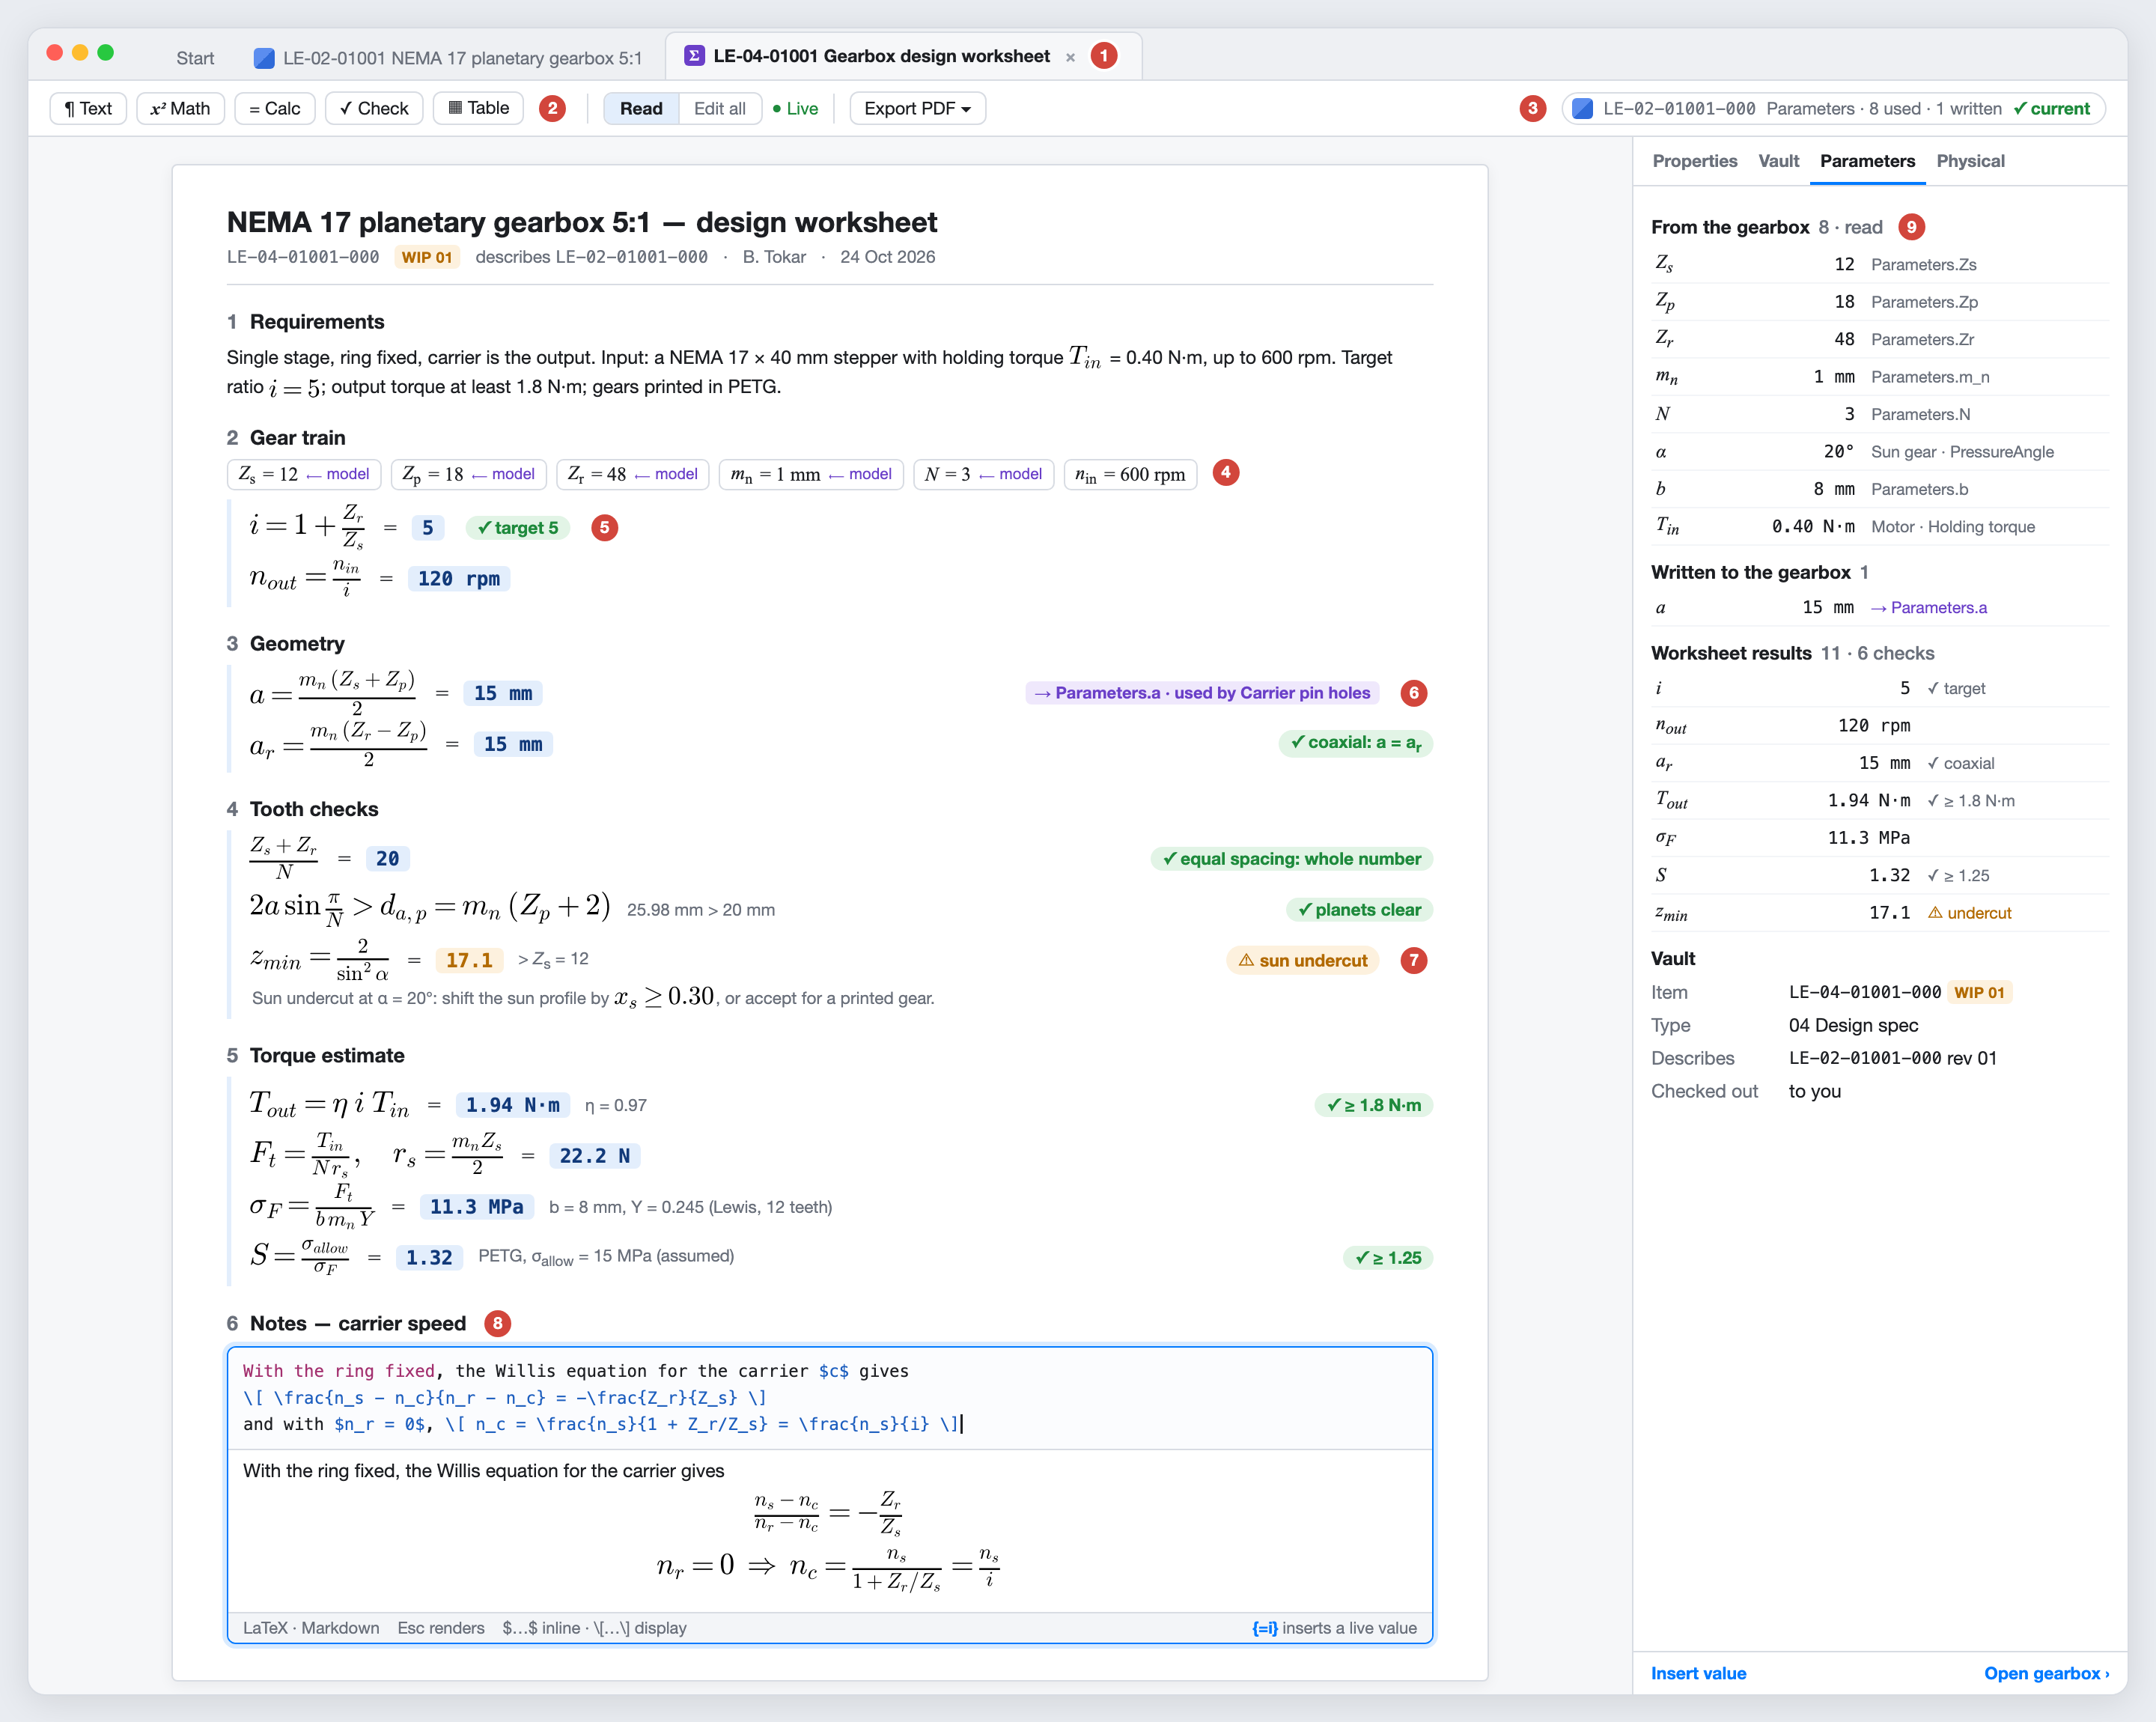
\includegraphics[width=\linewidth]{fig/mod15_sheet.png}}{\fbox{mod15\_sheet.png}}
\caption{Mock: the gearbox worksheet as a document tab (light). The formulas are drawn by matplotlib's mathtext, the
renderer the worksheet would use, so the figure shows the real look. The numbers match the table below.}
\label{fig:mod15-sheet}
\end{figure}

\begin{center}
\small
\begin{tabularx}{\linewidth}{@{}cp{3.0cm}X@{}}
\toprule
\# & Element & Behaviour\\
\midrule
\marker{1} & Document tab & A worksheet opens as its own tab next to the model's, named by P/N and title, with a
  $\Sigma$ icon. Cmd-W, the tab menu and the Start page treat it like any document.\\
\marker{2} & Toolbar & Insert a Text, Math, Calc, Check or Table block. \emph{Read} shows the page; \emph{Edit all}
  shows every block's source. \emph{Live}: results follow the model. \emph{Export PDF} (built in, or via LaTeX when
  installed).\\
\marker{3} & Link chip & The linked assembly, how many of its values the sheet reads and writes, and its state:
  \emph{current}, \emph{model changed} (orange) or \emph{not open}. A click opens the gearbox.\\
\marker{4} & Inputs & Names the sheet reads from the model, shown as chips with ``$\leftarrow$ model''; values typed in
  the sheet (here $n_{in}$) have no tag.\\
\marker{5} & Calc line & The source line \code{i = 1 + Zr / Zs} shows as an equation, then \textbf{= 5}. A check on
  the line shows \textcolor{bwgreen}{\checkmark} or a warning. Click a line to edit its source.\\
\marker{6} & Written to the model & \code{a = m\_n * (Zs + Zp) / 2 => Parameters} writes $a$ into the gearbox's
  Parameters sheet; the badge says who uses it (the carrier's pin holes).\\
\marker{7} & Warning & A check can warn rather than fail: the 12-tooth sun is below $z_{min} = 17.1$ for
  $\alpha = 20^\circ$, so it undercuts unless its profile is shifted. A real finding for the gearbox.\\
\marker{8} & LaTeX text & A text block in edit mode: Markdown with \code{\$\ldots\$} and \code{\textbackslash[\ldots\textbackslash]};
  the preview renders below; \code{\{=i\}} puts a live value into the prose.\\
\marker{9} & Right panel & With a worksheet tab active, the Parameters tab lists what the sheet reads, what it
  writes and its results; the Vault section shows the item and what it describes.\\
\bottomrule
\end{tabularx}
\end{center}

%----------------------------------------------------------------------
\subsubsection*{1. What the spikes showed (24 Oct)}

Four spikes in this build (FreeCAD~1.1.4-bw.1, Qt~6.8.3, PySide6~6.8.3, Python~3.11), three headless with
\code{FreeCADCmd} and one in the GUI (\file{worksheet-plan/spike\_units*.py}, \file{spike\_gui.py},
\file{spike\_pdf.py} in the agents' scratch folder).

\paragraph{Rendering.}
\begin{center}
\small
\begin{tabularx}{\linewidth}{@{}>{\raggedright\arraybackslash}p{3.6cm}X@{}}
\toprule
Check & Result\\
\midrule
Qt WebEngine & \textbf{Not in the build}: no \code{libQt6WebEngine*}, and \code{PySide6.QtWebEngineWidgets} does not
  import. QtPdf is missing too. So no KaTeX/MathJax in a web view.\\
What is there & \code{QtSvg}/\code{QtSvgWidgets}, \code{QtQml}/\code{QtQuick}, \code{QtPrintSupport}, and
  \code{QTextDocument} with \code{setMarkdown} (a Markdown table in 0.1--0.4\,ms).\\
Python packages & matplotlib~3.10.8, sympy~1.14, numpy, docutils, jinja2, lxml, Pillow. \textbf{Not}: pint, ziamath,
  markdown, mistune, latex2mathml, pygments; sympy's LaTeX \emph{parser} needs antlr4 (missing).\\
matplotlib mathtext & Renders $\backslash$frac, sub/superscripts, Greek, $\backslash$sqrt, $\backslash$sum,
  $\backslash$int, $\backslash$sin to SVG in \textbf{3--7\,ms} per formula (the first one 45\,ms in the GUI, 0.8\,s
  headless: font cache). Computer Modern via \code{mathtext.fontset = cm}. A subset of LaTeX:
  \code{\textbackslash begin\{cases\}} (and \code{align}, matrices) \textbf{fail}.\\
Formulas in a \code{QTextBrowser} & As image resources (SVG drawn to a 2$\times$ \code{QImage}) they show in a document
  tab (figure~\ref{fig:mod15-spike}). A custom \code{QTextObjectInterface} handler registers from Python but Qt
  \textbf{never calls it} (0 calls), so vector math inside a \code{QTextDocument} is out of reach from Python.\\
PDF & \code{QTextDocument.print\_} to \code{QPdfWriter}: 16\,ms, but the formulas go in as raster images. Drawing
  the SVG with \code{QSvgRenderer} on a \code{QPdfWriter} painter gives \textbf{vectors} (486 curves, 0 images) and real
  text (\code{Tj}).\\
TeX on your Mac & TeX Live 2026 (\file{/usr/local/texlive}, 9.7\,GB): \code{latexmk}, \code{pdflatex},
  \code{lualatex}, \code{xelatex}, \code{dvisvgm}, \code{dvipng}. \code{latex} + \code{dvisvgm} renders a formula with
  \code{cases} in \textbf{1.7\,s}. Most users of a FreeCAD build will not have TeX.\\
\bottomrule
\end{tabularx}
\end{center}

\begin{figure}[!htbp]
\centering
\IfFileExists{fig/mod15_spike.png}{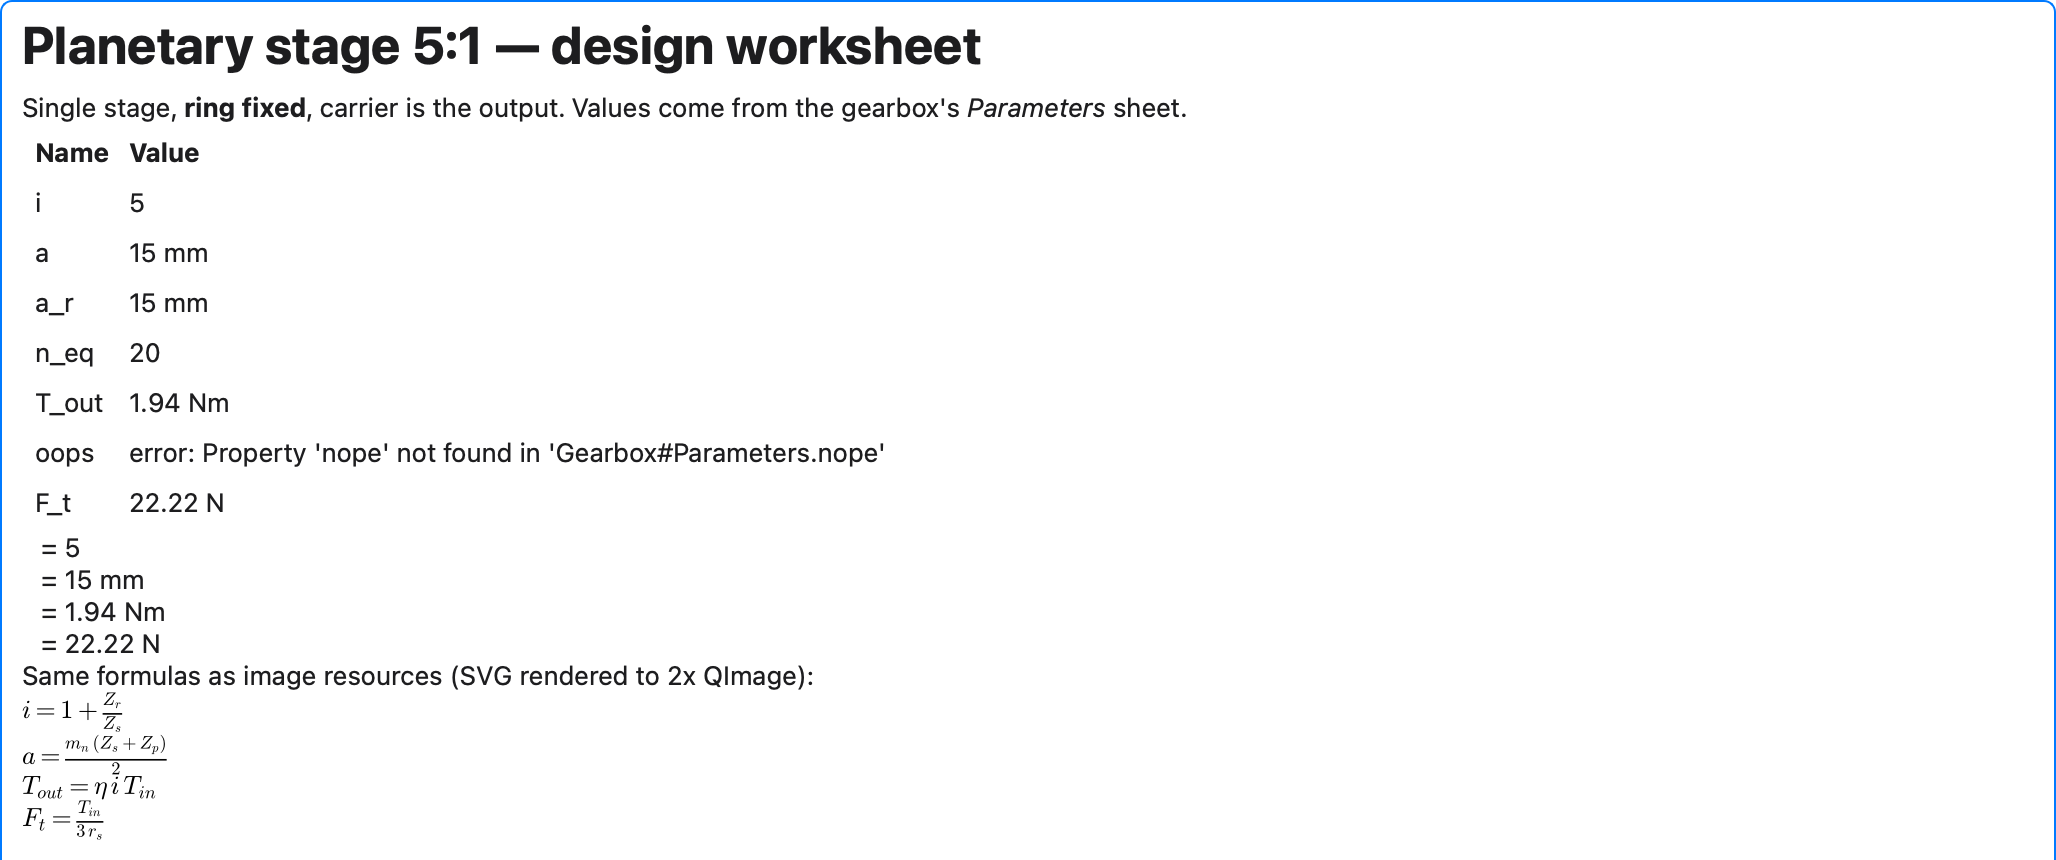
\includegraphics[width=0.7\linewidth]{fig/mod15_spike.png}}{\fbox{mod15\_spike.png}}
\caption{The GUI spike: a worksheet tab in this build. Values computed from the gearbox's Parameters through FreeCAD's
expression engine (one line fails on its own and the rest still compute); formulas from mathtext as image resources.
The empty lines above them are the custom text-object handler, which Qt never called.}
\label{fig:mod15-spike}
\end{figure}

\paragraph{Units and expressions.}
\begin{center}
\small
\begin{tabularx}{\linewidth}{@{}>{\raggedright\arraybackslash}p{3.6cm}X@{}}
\toprule
Check & Result\\
\midrule
\code{Units.Quantity} & Parses \code{0.4 N*m}, \code{3/4 in}, \code{200 mA}, \code{1 g/cm\^{}3}, \code{1 1/min};
  arithmetic keeps dimensions ($2\,\mathrm{N\,m} / 15\,\mathrm{mm} = 133.33\,\mathrm{N}$); \code{1 mm + 1 N} raises
  ``Unit mismatch''; \code{getValueAs("N*mm")} converts. Units have a type name (\code{Moment}, \code{Force}).\\
Expression grammar & The one in features, spreadsheets and \code{evalExpression}. It differs from the
  Quantity parser: \code{0.4 N*m}, \code{400 N*mm}, \code{1 kNm}, \code{1 Nmm}, \code{1 kg*m\^{}2} \textbf{fail to
  parse}; \code{0.4 Nm}, \code{1 N/mm\^{}2}, \code{1 kg/m\^{}3}, \code{1 rad/s}, \code{12 V * 1.7 A},
  \code{0.4 * 1 N * 1 m} work. A product of units after a number is the gap; quotients are fine. No \code{rpm}
  (\code{1000 / 1 min} works). Functions: \code{sqrt}, \code{cos(20 deg)}, \code{atan2}, \code{round}, \code{mod},
  \code{max}, \code{?:}, \code{pi}, \code{e}; \code{1 mm / 0} gives \code{inf mm}.\\
Spreadsheet aliases & \textbf{A unit or constant cannot be a name}: \code{m}, \code{mm}, \code{N}, \code{s},
  \code{in}, \code{A}, \code{g}, \code{T}, \code{pi}, \code{e} are refused (``Invalid alias''); \code{i}, \code{a},
  \code{m\_n}, \code{T\_in}, \code{alpha} are fine. Engineers' $m$ (module) and $T$ (torque) need another spelling.
  A cell \code{=0.40 N*m} is kept as \emph{text}, silently, and breaks every expression that uses it.\\
Display & \code{UserString} picks units well for N, N$\cdot$m (``1.90 Nm''), W, but shows MPa as ``2000.00 kPa''; a
  worksheet needs its own display unit per line.\\
\code{evalExpression} & \code{obj.evalExpression("1 + Parameters.Zr / Parameters.Zs")} gives 5.0 with no property
  and no recompute. \textbf{Cross-document} names work: \code{Gearbox\#Parameters.m\_n * (\ldots) / 2} = 15\,mm from
  another document.\\
Holding results & A worksheet value kept on a \code{VarSet} so that later lines can name it:
  \code{PropertyQuantity} refuses a value with a unit (``Not matching Unit!''); \code{PropertyPythonObject} holding a
  \code{Quantity} works (\code{p * 2}, \code{p + 1 mm}). Binding all lines as expressions on \emph{one} object: one bad
  line marks the object Invalid and \textbf{no} line gets a value. One \code{VarSet} per line isolates errors.\\
Change and cost & An observer's \code{slotRecomputedDocument} re-evaluated $i$ to 6 when $Z_r$ became 60. 200 chained
  lines recompute in 2.3\,ms; 7 lines evaluate in 0.4\,ms.\\
Cycles & A binding that closes a loop through the Parameters sheet is refused at \code{setExpression} (``cyclic
  reference'').\\
Model reads a value & A cylinder's radius bound to \code{Worksheet.a} took 15\,mm, and followed $m_n = 2$\,mm to
  30\,mm in one recompute; expressions on dynamic properties survive save and reload.\\
Sheet errors & One bad cell (\code{=nope * 2}) leaves the others computed (\code{after\_bad} = 24), but marks the whole
  sheet Invalid.\\
Context document & A plain \code{App.newDocument} for the evaluation context shows up as a tab
  (\emph{WorksheetCtx}); it must be made hidden and temporary.\\
\bottomrule
\end{tabularx}
\end{center}

\paragraph{What to reuse.} The Parameters tab (\file{bruceworx\_parameters.py}: the \emph{Parameters} sheet, columns
Name, Value, Comment, aliases, one undo step per edit), the right panel's \code{register(key, factory)}
(\file{bruceworx\_rightpanel.py}), the MDI page pattern of the vault settings page (\code{mdi.addSubWindow}), the
document-tab naming of \file{bruceworx\_doctabs.py}, the vault's \code{create\_item}/check-in and PDM-09's
\code{made\_from}, and the Claude Code bridge (\file{bruceworx\_bridge\_tools.py}, which already has
\code{set\_parameter}, consent and one undo step per call).

%----------------------------------------------------------------------
\subsubsection*{2. The design}

\paragraph{A worksheet is a text file.} One file per worksheet, \file{<P/N>.bwsheet}: Markdown with a short header, LaTeX
math in \code{\$\ldots\$} and \code{\textbackslash[\ldots\textbackslash]}, and fenced \code{calc} blocks. It diffs line by
line in the vault and in git, Claude can read and write it, and any editor opens it. Results are written into the
header at save so that a revision shows what was computed without FreeCAD. Not an \file{.FCStd}: a zip of XML would
hide the text from every diff.
\begin{lstlisting}
---
bw-worksheet: 1
pn: LE-04-01001-000
title: NEMA 17 planetary gearbox 5:1 - design worksheet
describes: LE-02-01001-000          # bare names are read from its Parameters sheet
results: {i: "5", a: "15 mm", T_out: "1.94 N*m", S: "1.32"}   # written at save
---
## 1 Requirements
Single stage, ring fixed, carrier is the output. Holding torque $T_{in}$ = {=T_in}.

## 2 Gear train
```calc
n_in = 600 / 1 min                   in rpm
i = 1 + Zr / Zs                      check i == 5 "target 5"
n_out = n_in / i                     in rpm
a = m_n * (Zs + Zp) / 2              in mm  => Parameters
a_r = m_n * (Zr - Zp) / 2            in mm  check a == a_r "coaxial"
z_min = 2 / sin(alpha)^2             warn z_min > Zs "sun undercut"
```
With the ring fixed, the Willis equation gives \[ n_c = \frac{n_s}{1 + Z_r/Z_s} \]
\end{lstlisting}

\paragraph{The calc language is FreeCAD's.} A line is \code{name = expression}, optionally followed by
\code{in <unit>} (display unit), \code{=> Parameters} (write to the model) and \code{check}/\code{warn <condition>
"<label>"}. The expression is FreeCAD's own grammar, so whatever works in a Pad's length works here and an exported line
can be copied into the Parameters sheet verbatim. The worksheet closes the gaps the spike found with three rewrites
before evaluation, each tested: a number followed by a \emph{product} of units (\code{0.4 N*m}) becomes
\code{(0.4 * 1 N * 1 m)}; \code{rpm} becomes \code{/ 1 min} (times $2\pi$ for an angular speed in \code{rad/s});
and a name that is a unit (\code{m}, \code{T}) is refused with a suggestion (\code{m\_n}, \code{T\_in}).
Names display as math: an underscore is a subscript (\code{T\_out} $\to T_{out}$), Greek names become letters
(\code{alpha} $\to \alpha$, \code{sigma\_F} $\to \sigma_F$).

\paragraph{How a name is found.} In this order: a name defined \emph{above} in the worksheet; an alias of the linked
model's \emph{Parameters} sheet (\code{Zr} $\to$ \code{<model>\#Parameters.Zr}, the chips marked ``$\leftarrow$
model''); an explicit path to any object's property (\code{Motor.HoldingTorque}, \code{Sun\_gear.PressureAngle});
FreeCAD's constants. A name found nowhere is an error on that line only.

\paragraph{Theory: evaluation order and errors.} Let the calc lines be $L_1,\dots,L_n$ in reading order, and let line
$L_k$ read the set $R_k$ of names. A worksheet may only read names defined \emph{above} it (as Mathcad does), so the
``reads'' graph has edges $L_j \to L_k$ only for $j<k$: reading order is a topological order by construction, and no
cycle can form inside a sheet. Each line is evaluated on its own, with the results above it in scope, so the cost is
$O(n)$ evaluations of a few microseconds each. A failing line $L_e$ poisons exactly the lines that depend on it,
the forward closure
\[
  P(e) = \{e\} \cup \{\,k > e : R_k \cap \mathrm{names}(P(e)) \ne \varnothing\,\},
\]
which are shown as ``depends on line $e$'' rather than with their own error; every other line still computes. The
spike shows why this needs our own loop: bound as expressions on one object, one bad line stops all of them.

\paragraph{Theory: units.} A quantity is a pair $(v, \mathbf d)$ of a value in base units (mm, kg, s, A, K, mol, cd,
and the angle) and a dimension vector $\mathbf d \in \mathbb Z^8$ (\code{Unit.Signature}). Products add dimension
vectors, quotients subtract them, sums need equal vectors, and a function such as $\sin$ needs $\mathbf d = \mathbf 0$
(or an angle). So $T_{out} = \eta\,i\,T_{in}$ has $\mathbf d(T_{out}) = \mathbf 0 + \mathbf 0 + (2,1,-2,0,\dots) =$
torque; a line \code{in MPa} on it is refused because $\mathbf d(\mathrm{MPa}) = (-1,1,-2,0,\dots) \neq \mathbf
d(T_{out})$. Display converts $v$ to the chosen unit $u$ as $v/v_u$; a check \code{a == a\_r} compares with a
relative tolerance of $10^{-9}$, so 15\,mm computed two ways is equal.

\begin{figure}[!htbp]
\centering
\begin{tikzpicture}[>=Stealth,
  box/.style={draw=black!30,rounded corners=3pt,fill=white,align=left,font=\footnotesize,inner sep=5pt,text width=4.9cm},
  lab/.style={font=\scriptsize\color{bwgrey},align=center}]
\node[box] (m) at (0,0) {\textbf{Gearbox}\\ \code{LE-02-01001-000.FCStd}\\[2pt]
  \emph{Parameters} sheet: \code{Zs Zp Zr m\_n N b a}\\ gears; carrier pin holes \code{= Parameters.a}};
\node[box] (w) at (10.4,0) {\textbf{Worksheet}\\ \code{LE-04-01001-000.bwsheet}\\[2pt]
  text, LaTeX, calc lines\\ results in its header};
\node[box,fill=black!3,text width=4.2cm] (c) at (10.4,-2.5) {hidden context document\\ (one \code{VarSet}, values per line)};
\node[box,fill=black!3,text width=7.6cm] (v) at (5.2,-4.4) {\textbf{Vault} journal: a check-in per file;\\
  a model check-in records its Parameters values $v(x)$;\\ a worksheet check-in records what it read, $r_W(x)$};
\draw[->,bwblue,thick] ([yshift=4mm]m.east) -- node[lab,above,text=bwblue] {reads bare names; re-evaluates\\ after each recompute (a few ms)} ([yshift=4mm]w.west);
\draw[->,bwred!80!black,thick] ([yshift=-4mm]w.west) -- node[lab,below,text=bwred!80!black] {\code{=> Parameters}: writes the\\ expression into the sheet,\\ one undo step} ([yshift=-4mm]m.east);
\draw[->,black!45] (w) -- node[lab,right] {evaluate} (c);
\draw[->,black!45,dashed] (m.south) |- (v.west);
\draw[->,black!45,dashed] (w.east) -- ++(0.35,0) |- (v.east);
\end{tikzpicture}
\caption{The data flow. The model never reads the worksheet file; a value the model needs is written into its own
Parameters sheet, where FreeCAD's recompute graph owns it.}
\label{fig:mod15-flow}
\end{figure}

\paragraph{Linking both ways.} \emph{Reading} is the name lookup above, live. \emph{Writing} is only through the
model's Parameters sheet: \code{=> Parameters} on a line puts the line's expression in the sheet (row \emph{a},
comment ``from LE-04-01001-000''), its worksheet names replaced by their Parameters aliases (a name that is not in the
sheet is offered for export too, or inlined as a value). It is one undo step in the model document, needs the model
checked out, and the Parameters tab shows the row as owned by the worksheet (edits there warn). \emph{Why not let a
feature read the worksheet directly?} The spike shows it works inside one document (\code{Worksheet.a} drove a
radius), but the worksheet is a separate file: a feature reading it and the worksheet reading the model would make a
cycle across files that FreeCAD's recompute cannot order (it orders only within its dependency graph, see \eref{MOD-02}), and the model would be stale by one evaluation after each change. Writing into the sheet keeps
the model's graph complete and acyclic and the model file self-contained: it opens and recomputes without the
worksheet.

\paragraph{Recalculation.} With \emph{Live} on, the worksheet listens to the documents it is linked to
(FreeCAD's \code{slotRecomputedDocument}) and re-evaluates (debounced 200\,ms; the gearbox sheet takes about 1\,ms). The link
chip turns orange while the model is not open (values are the last saved results, in grey). F9 re-evaluates by hand.
The context is a hidden, temporary document (\code{App.newDocument} with \code{hidden} and \code{temp} set) holding one
\code{VarSet} whose \code{PropertyPythonObject}s carry the values (spike: the only property type that takes any unit).

\paragraph{The tab.} A scroll area of block widgets in an MDI sub-window, not one \code{QTextDocument}: \emph{text}
blocks are \code{QTextBrowser}s fed with Markdown, inline math as image resources; \emph{math} and \emph{calc} blocks
paint their SVG formulas with \code{QSvgRenderer} (vector, any zoom). A calc line becomes LaTeX through a small printer
over FreeCAD's expression tree that keeps your order of terms (sympy's \code{latex} reorders: \code{1 + Zr/Zs} came
out as \code{\textbackslash frac\{Zr\}\{Zs\} + 1}). Formula SVGs are cached by the hash of their LaTeX. Click a block to
edit its source (figure~\ref{fig:mod15-sheet}, \marker{8}); Esc renders it. Light and dark follow the Vector Labs tokens.
\emph{Math beyond mathtext} (\code{cases}, \code{align}, matrices): when \code{latex} and \code{dvisvgm} are found, the
block is rendered by TeX (about 1.7\,s, cached); otherwise it shows its source with ``needs a TeX installation''.

\paragraph{PDF.} \emph{Export PDF} paints the blocks with the same code onto a \code{QPdfWriter} (A4 or Letter by the
project's units), with a title block (P/N, revision, state, what it describes, date): vector formulas, no TeX needed.
\emph{Export LaTeX} writes a \file{.tex} with the results filled in; \emph{PDF via LaTeX} runs \code{latexmk} on it when
found, for full LaTeX quality (your Mac has it).

\paragraph{The vault.} A new document type \code{04 Design spec} in the vault's \file{document\_types.json} (the
Vector vault has 01--03 today; Vault Settings adds it), a new item type \code{spec} in \file{pdm.py}'s
\code{ITEM\_TYPES}, and a \code{describes} field on \code{create\_item}, like a drawing's \code{drawing\_of}. The work
file is \file{<P/N>.bwsheet}, so \file{pdm\_workspace.py}'s fixed \code{SUFFIX = ".FCStd"} becomes a suffix per item
type (the PCB items of \eref{ECD-05} need the same). Check in, check out, revisions and release work as for any item; a
spec revises on its own (it is not dragged into the assembly's ECO, but the ECO lists it as affected). The project of
\eref{PDM-09} lists the spec under its top assembly in the Structure view, with its own state cell.

\paragraph{Theory: when is a worksheet out of date?} PDM-09 decides a drawing's state from the \emph{file versions} it was
made from. A worksheet can do better, because it knows the exact values it read. Let $I(W)$ be the inputs of worksheet
$W$ (every model name it read). At check-in, $W$ records $r_W = \{x \mapsto \text{value of } x\}$ for $x \in I(W)$; each
model check-in records the values $v(x)$ of its Parameters aliases (the FreeCAD side reads them at check-in, as PDM-09
records a fingerprint, so \file{pdm\_folder.py} stays free of FreeCAD). Then
\[
  \mathrm{state}(W) =
  \begin{cases}
    \text{out of date} & \text{if } \exists\, x \in I(W):\ |r_W(x) - v(x)| > 10^{-9}\,\max(|r_W(x)|, |v(x)|),\\
    \text{current} & \text{otherwise,}
  \end{cases}
\]
with $v$ taken from the latest check-in of the model (the released one for a released worksheet). A model change that
moves no value the worksheet reads (a fillet, a description) leaves it current; a change of $Z_r$ makes it out of date
and says which input moved (figure~\ref{fig:mod15-stale}). Inputs that are not in a Parameters sheet (an object's
property, such as the motor's torque) fall back to PDM-09's version rule and say so. As PDM-09's answer for drawings,
an out-of-date spec \emph{warns} in the release checklist of the assembly; it does not block.

\begin{figure}[!htbp]
\centering
\IfFileExists{fig/mod15_stale.png}{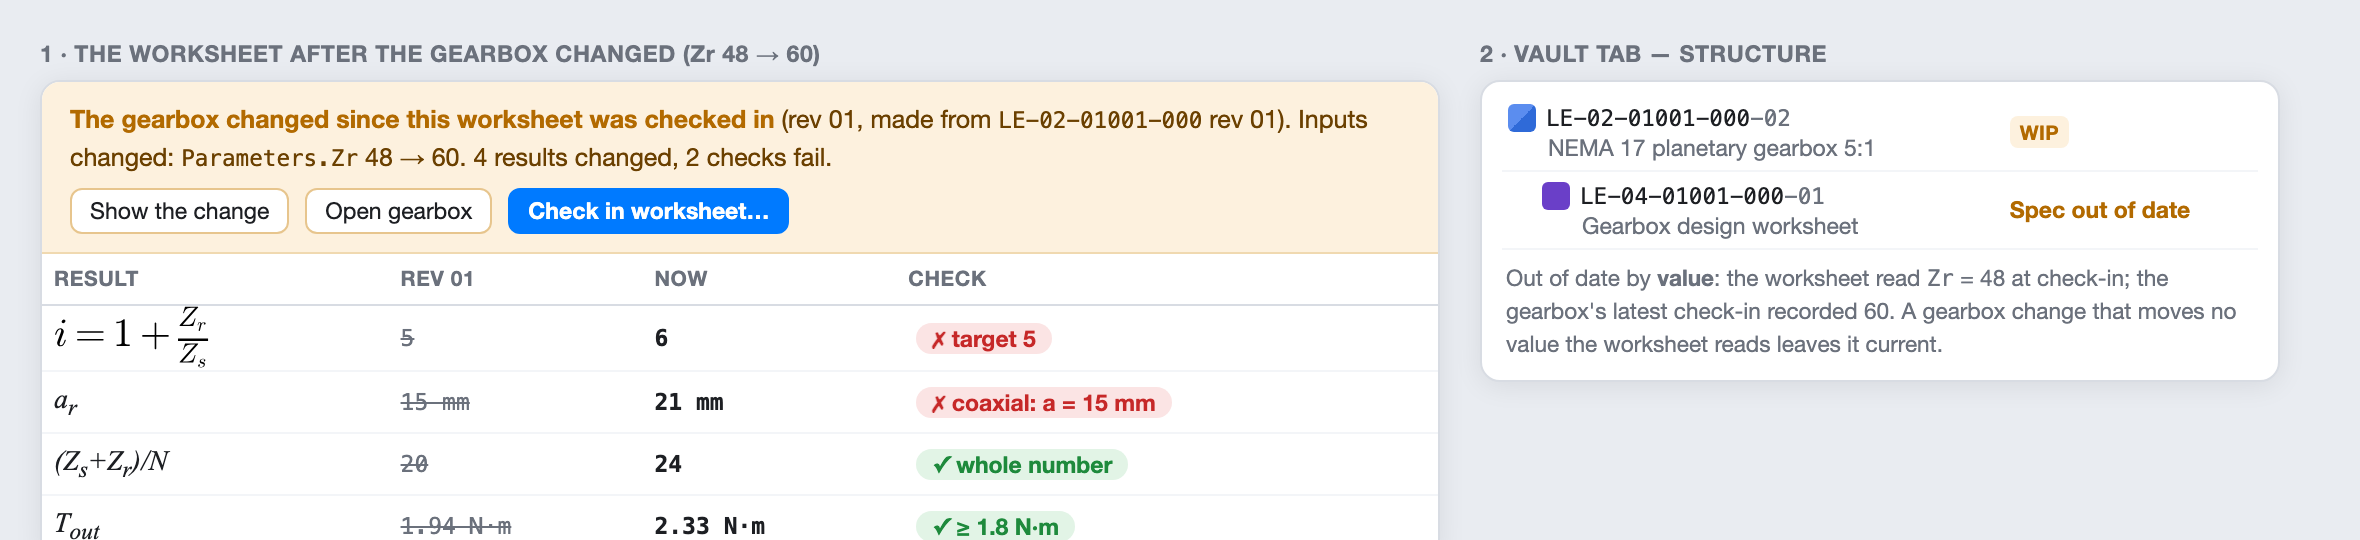
\includegraphics[width=\linewidth]{fig/mod15_stale.png}}{\fbox{mod15\_stale.png}}
\caption{Mock: after the gearbox changed $Z_r$ from 48 to 60 and was checked in. Left: the open worksheet's banner, with
what changed against its last revision and the checks that now fail. Right: the spec's row in the Structure view.}
\label{fig:mod15-stale}
\end{figure}

\paragraph{Claude.} Three bridge tools: \code{worksheet\_read} (the text and every line's value, unit and error),
\code{worksheet\_edit} (replace or insert a block by its heading, one undo step) and \code{worksheet\_eval} (evaluate an
expression in the worksheet's scope, nothing written). Same consent and log as the other tools. You can then ask
Claude ``add a bearing life check for the 683ZZ'' and see the block appear with its result.

%----------------------------------------------------------------------
\subsubsection*{3. Build order and effort}

\begin{center}
\small
\begin{tabularx}{\linewidth}{@{}lXl@{}}
\toprule
\# & Step & Effort\\
\midrule
1 & Engine, FreeCAD-free part: file format (header, blocks, \code{calc} lines), the three rewrites, name lookup,
  \code{in}/\code{=>}/\code{check}/\code{warn}, error closure; tests & 2\,d\\
2 & Engine, FreeCAD part: hidden context document, per-line \code{evalExpression}, cross-document names, display
  units, observer and debounce; headless tests on the gearbox numbers & 1.5\,d\\
3 & Math: expression-tree to LaTeX printer, mathtext SVG cache, TeX fallback when found; tests & 1.5\,d\\
4 & The tab: block widgets (text, math, calc, check, table), click to edit, toolbar, link chip, light and dark,
  open/save, Start page and Cmd-K entries & 3\,d\\
5 & Write to Parameters (\code{=>}), owned rows in the Parameters tab, the right panel's worksheet view, Insert
  value & 1.5\,d\\
6 & PDF: block painting on \code{QPdfWriter}, title block; Export LaTeX; PDF via \code{latexmk} & 1.5\,d\\
7 & Vault: type 04 Design spec, item type \code{spec} and \code{describes}, suffix per item type, check-in records
  ($r_W$, model values), state in the Structure view, release checklist line; contract tests & 2.5\,d\\
8 & Bridge tools for Claude; tests & 0.5\,d\\
9 & The Leonardo gearbox worksheet in the Vector vault, GUI checks, write-up & 1\,d\\
\midrule
 & Total & 15\,d\\
\bottomrule
\end{tabularx}
\end{center}
Steps 1--4 give a useful worksheet with no vault (saved as a file next to the model); 5--6 make it write and print; 7
waits for \eref{PDM-09}'s Structure view and is cheaper after \eref{ECD-05} makes the suffix per item type.

\paragraph{Risks.} \emph{Two grammars}: FreeCAD's expression grammar and its Quantity parser accept different unit
spellings; the rewrites cover what the spike found, and every rewrite is tested against both. \emph{A unit written
into a sheet cell} as \code{=0.40 N*m} silently becomes text and breaks what reads it; the export writes the rewritten
form, and the Parameters tab should flag text in a cell that looks like a quantity. \emph{mathtext is a subset of
LaTeX}: anything beyond it needs TeX, which most users will not have; the block then shows its source, never a wrong
rendering. \emph{Cross-document names} need the model open; the worksheet opens it hidden when needed, which costs
the model's load time (a second or two for the gearbox). \emph{Name clashes} between a worksheet name and a
Parameters alias: the worksheet's own definition wins and the chip says ``shadows model''. \emph{Upstream}: none of
this changes FreeCAD's C++; a proper vector text object (\code{QTextObjectInterface}) would need C++ and is not
needed with block widgets.

%----------------------------------------------------------------------
\subsubsection*{Questions before MOD-15 starts}

\begin{enumerate}
  \item \textbf{The file.} A Markdown text file \file{<P/N>.bwsheet} (diffable, readable anywhere), a JSON list of
        cells, or a FreeCAD document?\\
        \emph{Recommendation:} Markdown with a header and \code{calc} blocks, as above.
  \item \textbf{The calc syntax.} FreeCAD's expression grammar with \code{name = expr}, or Mathcad's \code{:=} for
        definitions and \code{=} for ``show the value''?\\
        \emph{Recommendation:} FreeCAD's grammar and \code{=}; every line shows its value anyway, and what you learn in
        the worksheet works in the Parameters tab and in features.
  \item \textbf{Order.} Lines may only use names defined above them (Mathcad, no cycles possible), or anywhere
        (spreadsheet-like)?\\
        \emph{Recommendation:} above only; the sheet reads as a derivation, top to bottom.
  \item \textbf{Names that are units.} Refuse \code{m} and \code{T} with a suggestion (\code{m\_n}, \code{T\_in}), or
        let the worksheet rename them behind the scenes?\\
        \emph{Recommendation:} refuse and suggest; a hidden rename would surprise you in the Parameters sheet.
  \item \textbf{Writing to the model.} Only through the Parameters sheet (\code{=> Parameters}), or may features read
        worksheet values directly?\\
        \emph{Recommendation:} only through Parameters (figure~\ref{fig:mod15-flow}); the model then opens and
        recomputes without the worksheet.
  \item \textbf{Out of date.} By the \emph{values} the worksheet read (exact), or by the model's \emph{version} (as for
        drawings)?\\
        \emph{Recommendation:} by values, falling back to the version where a value is not recorded.
  \item \textbf{Release.} Should an out-of-date spec block the assembly's release, or warn?\\
        \emph{Recommendation:} warn, as you chose for drawings in PDM-09.
  \item \textbf{Revisions.} Does the spec revise on its own, or move with the assembly in the same ECO?\\
        \emph{Recommendation:} on its own; an ECO that opens the assembly lists the spec as affected, ticked when its
        inputs changed.
  \item \textbf{Number.} \code{04 Design spec} with its own counter (\code{LE-04-01001-000} is simply the first), or
        the parent number of the assembly it describes?\\
        \emph{Recommendation:} its own counter, like drawings today (PDM-09 Q11); the \emph{describes} link and the
        Structure view connect them.
  \item \textbf{Several models.} One worksheet describes one assembly (and reads anything below it), or several
        unrelated models?\\
        \emph{Recommendation:} one; a second model's values are reachable by explicit path when needed.
  \item \textbf{Math rendering.} mathtext built in, TeX only when installed?\\
        \emph{Recommendation:} yes. Bundling a TeX would add hundreds of MB; KaTeX would need Qt WebEngine, which this
        build does not have.
  \item \textbf{Display units.} SI with N$\cdot$m and MPa as defaults (FreeCAD shows ``2000 kPa''), each line can say
        \code{in <unit>}?\\
        \emph{Recommendation:} yes, defaults per quantity type in the worksheet header, overridable per line.
  \item \textbf{Claude.} Let Claude edit worksheets through the bridge (with the usual consent, one undo step per
        block)?\\
        \emph{Recommendation:} yes; read and evaluate always, edit only with the consent given for the session.
  \item \textbf{Milestone.} \eref{MOD-15} at M2, after the gearbox is modelled?\\
        \emph{Recommendation:} yes, as you ranked it; steps 1--4 could start earlier if you want to write the gearbox
        worksheet while modelling it.
\end{enumerate}
